\documentclass[12pt]{book}

\usepackage[dvips,letterpaper,margin=0.75in,bottom=0.5in]{geometry}
\usepackage{cite}
\usepackage{slashed}
\usepackage{graphicx}
\usepackage{amsmath}
\usepackage{latexsym,amssymb,amsmath}




\usepackage[american,fulldiode]{circuitikz}
\tikzset{component/.style={draw,thick,circle,fill=white,minimum size =0.75cm,inner sep=0pt}}

\begin{document}
\ctikzset{bipoles/thickness=1}
\ctikzset{bipoles/length=.6cm}

\title{Lecture Notes:  RLC Circuits}
\author{Michael Mulhearn}

\maketitle

\chapter{Direct Current Circuits and Resistance}

\section{The Electric Field}

Suppose there are two particles of charge $q_1$ and $q_2$ located a distance $r$ apart.
The force on particle 2 is given by:
\begin{displaymath}
\vec{F}_{21} = k_e \frac{q_1 q_2}{r^2} \cdot \hat{r}_{21}
\end{displaymath}
where $k_e$ is Coulomb's constant and $\hat{r}_{21}$ is a unit vector pointing from particle 1 to particle 2.

Now consider the force $\vec{F}$ on a particle of charge $Q$ due to $N$ particles, which will be the sum:
\begin{displaymath}
\vec{F} = Q \, k_e \, \sum_{i=1}^N \frac{q_i}{r_{i}^2} \hat{r}_{i}
\end{displaymath}
where $r_i$ is the distance between the particle of charge $Q$ and the $i$th particle, and $\hat{r}_i$ is the unit vector pointing from the $i$th particle toward the charge $Q$.  If the charge $Q$ is small enough not to disturb the location of the $N$ other charges, then the ratio of the force $F$ to the charge $Q$ is independent of the charge $Q$, and we call this quantity the electric field:
\begin{displaymath}
\vec{E} \equiv \lim_{Q \to 0} \frac{\vec{F}}{Q}
\end{displaymath}
The importance of this distinction is that the electric field is due solely due to the source charges, independent of the particle of charge $Q$ experiencing the force.  The electric field exists whether or not anything is there to experience a force!  The force experienced by a particle of charge $Q$ in an electric field $\vec{E}$, we simply calculate:
\begin{displaymath}
\vec{F} = Q \vec{E}.
\end{displaymath}

\section{The Electric Potential}

For a conservative force the change in potential energy that results from moving a particle from $x=a$ to $x=b$ is defined as the negative of the work done by the conservative force:
\begin{displaymath}
U_{ba} \equiv -W_{\rm CSV} = - \int_a^b F_x \cdot dx
\end{displaymath}
As discussed above, the Coulomb force $\vec{F}$ experienced by a 
particle of charge $Q$ in an electric field $\vec{E}$ is given by:
\begin{displaymath}
\vec{F} = Q \vec{E} 
\end{displaymath}
which is a conservative force proportional to the charge $Q$.   If we consider moving a particle of charge $Q$ moving along the $x$-axis from $x=a$ to $x=b$, we can define a quantity $V_{ba}$ called the electric potential difference which is simply the change in potential energy divided by the charge of the particle:
\begin{displaymath}
V_{ba} \equiv \frac{U_{ba}}{Q}  = - \int_a^b E_x \cdot dx
\end{displaymath}
The unit of electrical potential difference is the Volt (V), where $1~\rm{V} = 1~\rm{J / C}$, and a difference in electrical potential is often informally referred to as simply the voltage.  This definition generalizes to three dimensions, but is tedious (you simply add additional identical integrals for $y$ and $z$) without vector calculus, which we won't use in this  course.   In this case the points $b$ and $a$ are simply any two points in space.

\begin{figure}[htbp]
\begin{center}
\begin{tabular}{ccc}
\begin{circuitikz}[line width=1pt]
\draw (0,0) to[battery1,bipoles/length=1.5cm] ++(0,+2.0);
\draw (0,0.7) node[left]{$-$};
\draw (0,1.4) node[left]{$+$};
\end{circuitikz} &  
\begin{circuitikz}[line width=1pt]
\draw (0,0) to[battery,bipoles/length=1.5cm] ++(0,+2.0);
\draw (0,0.5) node[left]{$-$};
\draw (0,1.6) node[left]{$+$};
\end{circuitikz} & 
\begin{circuitikz}[line width=1pt]
\draw (0,0) to[voltage source,bipoles/length=1.5cm] ++(0,+2.0);
\end{circuitikz} \\
(a) & (b) & (c) \\
\end{tabular}
\end{center}
\caption{The circuit diagram for (a) voltage cell, (b) battery, (c) voltage source.  The $+$ and $-$ symbols are usually omitted from (a) and (b).  Often, symbol (a) is used to indicate a generic voltage source, even when (c) would be more appropriate.}
\label{fig:dcsymbols}
\end{figure}

The battery is a frequently encountered electrical component that imposes a constant electrical potential difference between two points (the two terminals of the battery).  Batteries are devices that exploit different chemical potentials of two metals.  A cell consisting of zinc and copper will have a characteristic voltage of $1.1~\rm V$.  To build batteries of different voltages, multiple cells can be combined.  In lab, you will use a bench-top DC voltage supply, a more complicated piece of equipment that uses electrical power provided by the wall outlets to maintain a fixed voltage between its terminals.  All real devices have limitations.  For instance, batteries drop in voltage as they become discharged.  

Because these devices supply a fixed voltage which is approximately constant with time, they produce circuits with currents in one direction only.   As a result, these are called direct current (DC) sources.
The electrical symbols for various DC voltage sources are shown in Fig.~\ref{fig:dcsymbols}

\begin{figure}[htbp]
\begin{center}
\begin{tabular}{cc}
\begin{circuitikz}[line width=1pt]
\draw (0,0) node[ground,yscale=2.0]{};
\end{circuitikz}  & 
\begin{circuitikz}[line width=1pt]
\draw (0,0) coordinate(A) to[voltage source,bipoles/length=1.5cm,l_=3~\rm V] ++(0,+2.0)
coordinate(B) to[voltage source,bipoles/length=1.5cm,l_=2~\rm V] ++(0,+2.0) coordinate(C);
\draw (A) to[short,-o] ++(1.0,0) node[right]{A};
\draw (B) to[short,-o] ++(1.0,0) node[right]{B};
\draw (C) to[short,-o] ++(1.0,0) node[right]{C};
\draw (A) node[ground,yscale=2.0]{};
\end{circuitikz} \\
(a) & (b) \\
\end{tabular}
\end{center}
\caption{The (a) ground symbol, and (b) circuit diagram for two voltage sources connected in series and referenced to ground.}
\label{fig:poteg}
\end{figure}

By definition, a conservative force has a single value for the relative potential $U_{ba}$ which is independent of the path taken from point $a$ to point $b$.   The same holds for $V_{ba}$.
This implies that $V_{ab} = -V_{ba}$ which is why terminals of any voltage source have a polarity.  If we specify a reference point, we can define the electrical potential as the electrical potential difference of the point of interest and the reference point.   Most often, the reference point chosen is the earth ground, which has it's own symbol, shown in Fig.~\ref{fig:poteg}a.  In the circuit diagram of Fig.~\ref{fig:poteg}b, examples of electrical potential differences are $V_{\rm BA} = 3~{\rm V}$, $V_{\rm BC} = 2~{\rm V}$,  and $V_{\rm AB}= -3~{\rm V}$, while examples of electrical potentials are $V_A = 0$, $V_B = 3~\rm V$ $V_C = 5~\rm V$.

\section{Conductors and Resistors}

The electric field in a perfect conductor is zero.  This implies that any two points connected by a perfect conductor are at the same electric potential, which we refer to as a short circuit.  As a practical matter, we treat very good conductors, such as copper, as if they were ideal conductors.  We create a short circuit by connecting any two points with a segment of copper wire.   Conductors allow charge to flow through them readily.   The amount of charge that passes through any electrical component per unit time is called the current $I$:
\begin{displaymath}
I = \frac{dQ}{dt}
\end{displaymath}
And is measured in Amperes (A) where $1~{\rm A} = 1 {\rm C / s}$.

Materials which do not readily conduct charge are called electrical insulators, and are used to protect components, such as wires, from accidental contact causing unintentional short circuits.  All materials eventually conduct electricity when the voltage is high-enough, and this imposes limits on the voltage that can be reached in practical circuits.

\begin{figure}[htbp]
\begin{center}
\begin{circuitikz}[line width=1pt]
\draw (0,0) to[battery,bipoles/length=1.5cm,l=$V$] ++(0,+3.0) to[short,i>=$I$] ++(3.0,0) coordinate(A)
to[resistor,l_=$R$] ++(0,-3.0) coordinate(B) to[short] ++(-3.0,0);
\draw (A) to[short,*-o] ++(1.0,0) node[right]{A};
\draw (B) to[short,*-o] ++(1.0,0) node[right]{B};
\end{circuitikz} 
\end{center}
\caption{A resistor connected to a battery.}
\label{fig:ohms}
\end{figure}

If we construct a composite material from a mixture of graphite (a conductor) and ceramic dust (an insulator) held together by a resin, we obtain a resistor: a device which has mobile charges that do not flow as readily as in a conductor.  When we connect a resistor to a battery,  as shown in Fig.~\ref{fig:ohms}, 
the battery imposes a non-zero electric potential across the resistor.  This implies that a non-zero electric field is present in the resistor.  This electric field exerts a force on the mobile electrons in the resistor, resulting in a net flow of electrons through the resistor.  Resistors have a characteristic resistance $R$ which relates the current $I$ that flows through the resistor to the voltage $V$ across it: 
\begin{displaymath}
V = I R
\end{displaymath}
This relationship is referred to as Ohm's Law, and the unit of resistance is the Ohm ($\rm \Omega$) where $1~{\rm \Omega} = 1~{\rm V / A}$.

\section{Kirchoff's Laws}

The circuits we have encountered so far are quite simple, containing at most a single closed loop with only one current to consider.  More complicated circuits can include multiple circuits.
Ultimately the behavior of the circuit is governed by the laws of electrostatics, but Kirchhoffs Laws conveniently cast the important results from electrostatics into a form that can be applied to any circuit.

\begin{figure}[htbp]
\begin{center}
\begin{circuitikz}[line width=1pt]
\draw (0,0) to[short,i>=$I_1$,-*] ++(1.4,1.4) coordinate(C);
\draw (C) to[short,i>=$I_3$] ++(1.4,-1.4);
\draw (C) to[short,i<=$I_2$] ++(0,2);
\end{circuitikz} 
\end{center}
\caption{An example of Kirchoff's Current Law:  $I_1 + I_2 = I_3$}.
\label{fig:kcleg}
\end{figure}


The conservation of charge implies that the total current into a node must equal the total current out of a node.  If currents are all defined such that positive current is into the node, this law can be written simply as:
\begin{displaymath}
\sum_k I_k = 0.
\end{displaymath}
The electric field is conservative which implies that the net electric potential when traversing any closed loop is zero.  If the voltage drop across each electric component is defined in the direction of the closed loop, this law can be written simply as:
\begin{displaymath}
\sum_k V_k = 0.
\end{displaymath}
When determining the drop across a resistor from Ohm's law, one must remember the orientation of current and voltage (as in Fig.~\ref{fig:ohms}) when determining the sign.  You should be able to reason that when traversing a resistor in the same direction as the current, you drop in voltage (so add a term $-IR$ when using KVL).  When traversing a resistor in the opposite direction as the current, you rise in voltage (so add a term $IR$ when using KVL.) 

\begin{figure}[htbp]
\begin{center}
\begin{circuitikz}[line width=1pt]
\draw (0,0) to[battery,bipoles/length=1.5cm,l=$V$] ++(0,+3.0) to[resistor,l=$R_1$,i>=$I_1$] ++(3.0,0) coordinate(A) to[resistor,l=$R_2$,i>=$I_2$] ++(0,-3.0) coordinate(B) to[short] ++(-3.0,0);
\draw (A) to[R,*-,l=$R_3$,i>=$I_3$] ++(3.0,0) |- (B);
\draw (1.5,1.5) coordinate(L) node[scale=4]{$\circlearrowright$};
\draw (L) node[]{$1$};
\draw (4.5,1.5) coordinate(L) node[scale=4]{$\circlearrowright$};
\draw (L) node[]{$2$};
\end{circuitikz} 
\end{center}
\caption{An example of Kirchoff's Voltage Law.}
\label{fig:kvleg}
\end{figure}

For example, consider the circuit in Fig.~\ref{fig:kvleg}.  From KCL we obtain:
\begin{displaymath}
I_1 = I_2 + I_3
\end{displaymath}
while from KVL we traverse the loop labeled "1" to obtain:
\begin{displaymath}
0 = V  - I_1 R_1 - I_2 R_2
\end{displaymath}
and we traverse the loop labeled "2" to obtain
\begin{displaymath}
0 = I_1 R_1 - I_2 R_2
\end{displaymath}
Pay close attention to the signs of the voltage drops across the resistors and make sure you can reproduce them!



\section{Resistors in Series And Parallel}

\begin{figure}[htbp]
\begin{center}
\begin{tabular}{c@{\hskip 2cm}c}
\begin{circuitikz}[line width=1pt]
\draw (0,0) to[battery,bipoles/length=1.5cm,l=$V$] ++(0,+4.0) to[short, i>=$I$] ++(2.0,0) coordinate(A);
\draw (A) to[resistor,l_=$R_1$] ++(0,-2.0) to[resistor,l_=$R_2$] ++(0,-2.0) to[short] ++(-2.0,0);
\end{circuitikz} &
\begin{circuitikz}[line width=1pt]
\draw (0,0) to[battery,bipoles/length=1.5cm,l=$V$] ++(0,+4.0) to[short, i>=$I$] ++(2.0,0) coordinate(A);
\draw (A) to[resistor,l=$R_{\rm eq}$] ++(0,-4.0) to[short] ++(-2,0);
\end{circuitikz} \\
(a) & (b) \\
\end{tabular}
\caption{Resistor circuits showing (a) two resistors in series and (b) a single equivalent resistance $R_{\rm eq} = R_1 + R_2$ which produces the same current $I$.}
\label{fig:series}
\end{center}
\end{figure}

Consider the circuit in Fig.~\ref{fig:series} in which a current $I$ flows through to resistors $R_1$ and $R_2$ in series.  We can simplify this circuit by determining a single equivalent resistance $R_{\rm eq}$ which when installed in the circuit in place of $R_1$ and $R_2$ will result in the same current $I$.
Applying KVL to both circuits results in:
\begin{eqnarray*}
0 &=& V - I R_1 - I R_2 \\
0 &=& V - I R_{\rm eq} \\
\end{eqnarray*}
which can be solved to obtain:
\begin{displaymath}
R_{\rm eq} = R_1 + R_2.
\end{displaymath}
It is left as an exercise to show that for any number of resistors wired in series, the equivalent resistance
is given by:
\begin{equation} \label{eqn:rseries}
R_{\rm eq} = \sum_i R_i. 
\end{equation}

\begin{figure}[htbp]
\begin{center}
\begin{tabular}{c@{\hskip 2cm}c}
\begin{circuitikz}[line width=1pt]
\draw (0,0) to[battery,bipoles/length=1.5cm,l=$V$] ++(0,+4.0) to[short,i>=$I$] ++(2.0,0) coordinate(A);
\draw (A) to[resistor,l_=$R_1$,i>=$I_1$] ++(0,-4.0) to[short] ++(-2,0);
\draw (A) to[short,*-] ++(2.0,0.0) to[resistor,l_=$R_2$,i>=$I_2$] ++(0.0,-4.0) to[short,-*] ++(-2.0,0);
\end{circuitikz} &
\begin{circuitikz}[line width=1pt]
\draw (0,0) to[battery,bipoles/length=1.5cm,l=$V$] ++(0,+4.0) to[short,i>=$I$] ++(2.0,0) coordinate(A);
\draw (A) to[resistor,l=$R_{\rm eq}$] ++(0,-4.0) to[short] ++(-2,0);
\end{circuitikz} \\
(a) & (b) \\
\end{tabular}
\caption{Resistor circuits showing (a) two resistors in parallel and (b) a single equivalent resistance $R_{\rm eq}$ which produces the same total current $I$.}
\label{fig:parallel}
\end{center}
\end{figure}

Next consider the circuit in Fig.~\ref{fig:series} in which a total current $I$ is shared between two resistors $R_1$ and $R_2$.  Once again, we can simplify this circuit by determining a single equivalent resistance $R_{\rm eq}$ which when installed in the circuit in place of $R_1$ and $R_2$ will result in the same current $I$.  Applying KCL and KVL we determine:
\begin{eqnarray*}
I &=& I_1 + I_2 \\
0 &=& V - I_1 R_1 \\
0 &=& V - I_2 R_2 \\
0 &=& V - I R_{\rm eq} \\
\end{eqnarray*}
which can be solved to determine:
\begin{displaymath}
R_{\rm eq} = \frac{R_1 R_2}{R_1 + R_2}
\end{displaymath}
It is left as an exercise to show that for any number of resistors wired in series, the equivalent resistance
is given by:
\begin{equation} \label{eqn:rparallel}
\frac{1}{R_{\rm eq} }= \sum_i \frac{1}{R_i}. 
\end{equation}

\begin{figure}[htbp]
\begin{center}
\begin{tabular}{c@{\hskip 2cm}c}
\begin{circuitikz}[line width=1pt]
\draw (0,0) node[ground,yscale=2.0]{} to[battery,bipoles/length=1.5cm,l=$V$] ++(0,+4.0) to[short,i>=$I$] ++(2.0,0) coordinate(A);
\draw (A) to[resistor,l_=$R_1$] ++(0,-2.0) coordinate(B) to[resistor,l_=$R_2$] ++(0,-2.0) to[short] ++(-2.0,0);
\draw (B) to[short,*-o] ++(1.0,0) node[right]{$V_{\rm out}$};
\end{circuitikz} &
\begin{circuitikz}[line width=1pt]
\draw (0,0) node[ground,yscale=2.0]{} to[battery,bipoles/length=1.5cm,l=$V$] ++(0,+4.0) to[short,i=$I$] ++(2.0,0) coordinate(A);
\draw (A) to[resistor,l_=$R_1$,i>=$I_1$] ++(0,-4.0) to[short] ++(-2,0);
\draw (A) to[short,*-] ++(2.0,0.0) to[resistor,l_=$R_2$, i>=$I_2$] ++(0.0,-4.0) to[short,-*] ++(-2.0,0);
\end{circuitikz} \\
(a) & (b) \\
\end{tabular}
\caption{Resistors in series and in parallel used to implement a (a) voltage divider and a (b) current divider.}
\label{fig:dividers}
\end{center}
\end{figure}

The voltage divider circuit of Fig.~\ref{fig:dividers}a is a frequently encountered circuit.  The two resistors have an equivalent resistance $R_1 + R_2$ and so the current is:
\begin{displaymath}
I = \frac{V}{R_1 + R_2} 
\end{displaymath}
and the output voltage is the voltage drop across one resistor $R_2$, 
\begin{displaymath}
V_{\rm out} = I R_2 = \frac{R_2}{R_1 + R_2} V
\end{displaymath}
It is left as an exercise to show that the current divider circuit in Fig.~\ref{fig:dividers}b 
\begin{equation} \label{eqn:idivider}
\frac{I_1}{I_2} = \frac{R_2}{R_1}
\end{equation}

\section{The Superposition Principle}

In electrostatics, the superposition principle states that the electric field created at a point in space by a particular charge is independent of any other charges.  This principle allows us to simplify problems in electrostatics by considering the contribution from each charge in turn, constructing a partial solution for each charge while neglecting other charges, and constructing a solution from the sum of each partial solution.

In circuit analysis, the laws of electrostatics govern our circuits as well.  When considering a circuit with multiple voltage sources, we can consider one voltage source at a time, short circuiting other voltage sources.  The complete solution is simply the sum of each partial solution.

\section{Sources, Loads, and I-V Curves}

\begin{figure}[htbp]
\begin{center}
\begin{tabular}{ccc}
\begin{circuitikz}[line width=1pt]
\draw (0,0) node[right]{B} to[short,o-] ++(-1.0,0) to[battery,bipoles/length=1.5cm,l=$V$] ++(0,+4.0) to[short, i>=$I$,-o] ++(1.0,0) node[right]{A};
\end{circuitikz} &
\begin{circuitikz}[line width=1pt]
\draw (0,0) node[left]{B} to[short,o-] ++(1.0,0) to[R,l=$R_1$] ++(0,+4.0) to[short, i<=$I$,-o] ++(-1.0,0) node[left]{A};
\end{circuitikz} &
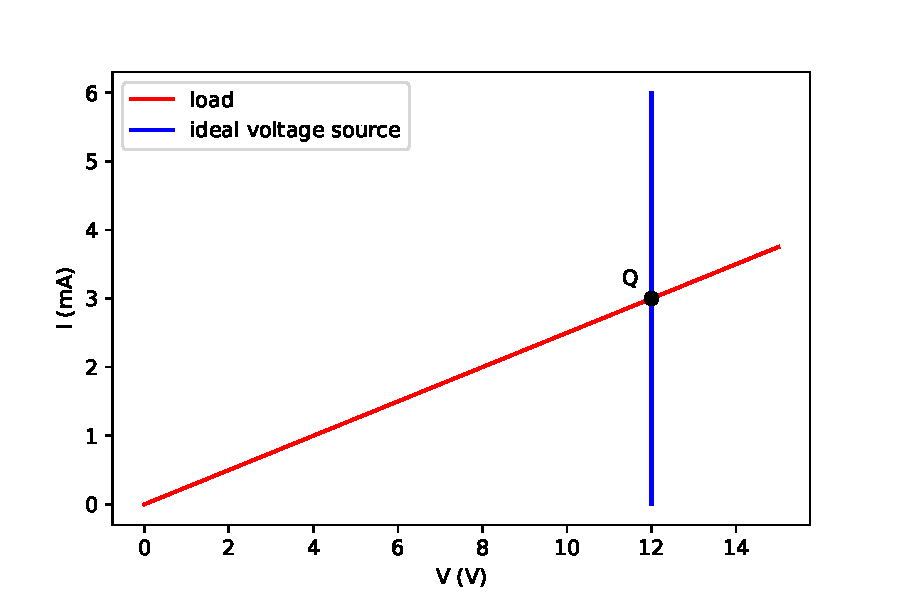
\includegraphics[height=0.3\textheight]{figs/thev_ideal.pdf} \\
(a) & (b) & (c) \\
\end{tabular}
\caption{ Electrical networks (a) for an ideal voltage source as source and (b) for a resistor as load, and (c) their corresponding $I-V$ curves.  The operating point for the circuit when the load is connected to the source is the intersection of these two curves.}
\label{fig:iv_ideal}
\end{center}
\end{figure}


\begin{figure}[htbp]
\begin{center}
\begin{tabular}{ccc}
\begin{circuitikz}[line width=1pt]
\draw (0,0) node[right]{B} to[short,o-] ++(-1.0,0) to[battery,bipoles/length=1.5cm,l=$V$] ++(0,+2.0) 
to[R, l=$R_{\rm src}$] ++(0,+2.0) to[short, i>=$I$,-o] ++(1.0,0) node[right]{A};
\end{circuitikz} &
\begin{circuitikz}[line width=1pt]
\draw (0,0) node[left]{B} to[short,o-] ++(1.0,0) to[R,l=$R_1$] ++(0,+4.0) to[short, i<=$I$,-o] ++(-1.0,0) node[left]{A};
\end{circuitikz} &
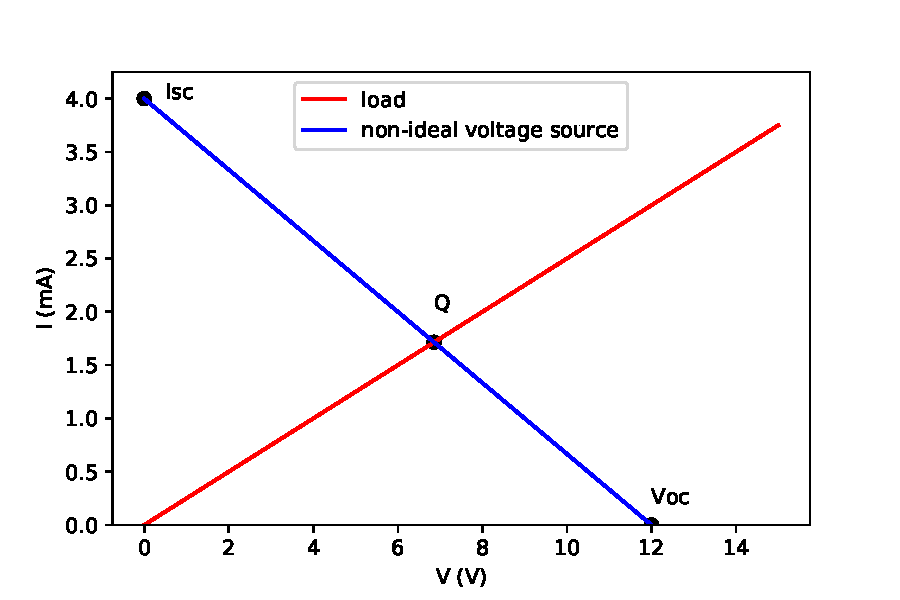
\includegraphics[height=0.3\textheight]{figs/thev_nonideal.pdf} \\
(a) & (b) & (c) \\
\end{tabular}
\caption{ Electrical networks (a) for a voltage source include source impedance and (b) for a resistor, and (c) their corresponding $I-V$ curves.  The operating point for the circuit when the load is connected to the source is the intersection of these two curves.}
\label{fig:iv_ideal}
\end{center}
\end{figure}



\section{Thevenin Equivalent Circuit}

\begin{figure}[htbp]
\begin{center}
\begin{tabular}{ccc}
\begin{circuitikz}[line width=1pt]
\draw (0,0) node[right]{B} to[short,o-] ++(-1.0,0) to[battery,bipoles/length=1.5cm,l=$V_{\rm th}$] ++(0,+2.0) 
to[R, l=$R_{\rm th}$] ++(0,+2.0) to[short, i>=$I$,-o] ++(1.0,0) node[right]{A};
\end{circuitikz} &
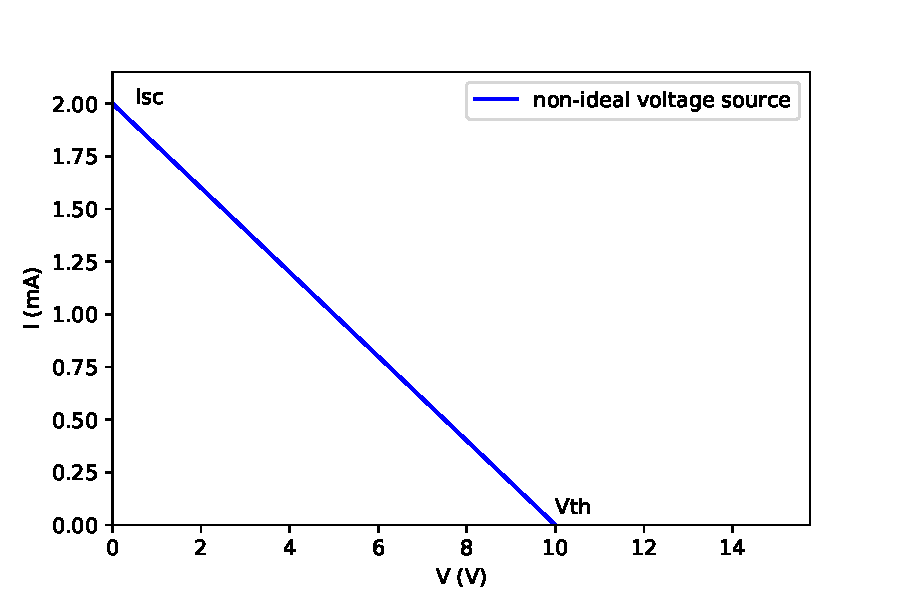
\includegraphics[height=0.3\textheight]{figs/thev.pdf} \\
(a) & (b) & (c) \\
\end{tabular}
\caption{ Electrical networks (a) for a voltage source include source impedance and (b) for a resistor, and (c) their corresponding $I-V$ curves.  The operating point for the circuit when the load is connected to the source is the intersection of these two curves.}
\label{fig:iv_ideal}
\end{center}
\end{figure}


\section{Exercises}

\begin{enumerate}

\item Derive Equations~\ref{eqn:rseries} and \ref{eqn:rparallel}.

\item Derive Equations~\ref{eqn:idivider}.

\end{enumerate}


\chapter{Alternating Current Circuits and Impedance}

\section{Capacitors}

\section{Inductors}




\end{document}




